\chapter{Use case}

%begin free user section
\section{Unidentified user}
	\subsection{Overview}
		\begin{figure}[ht]
			\begin{center}
				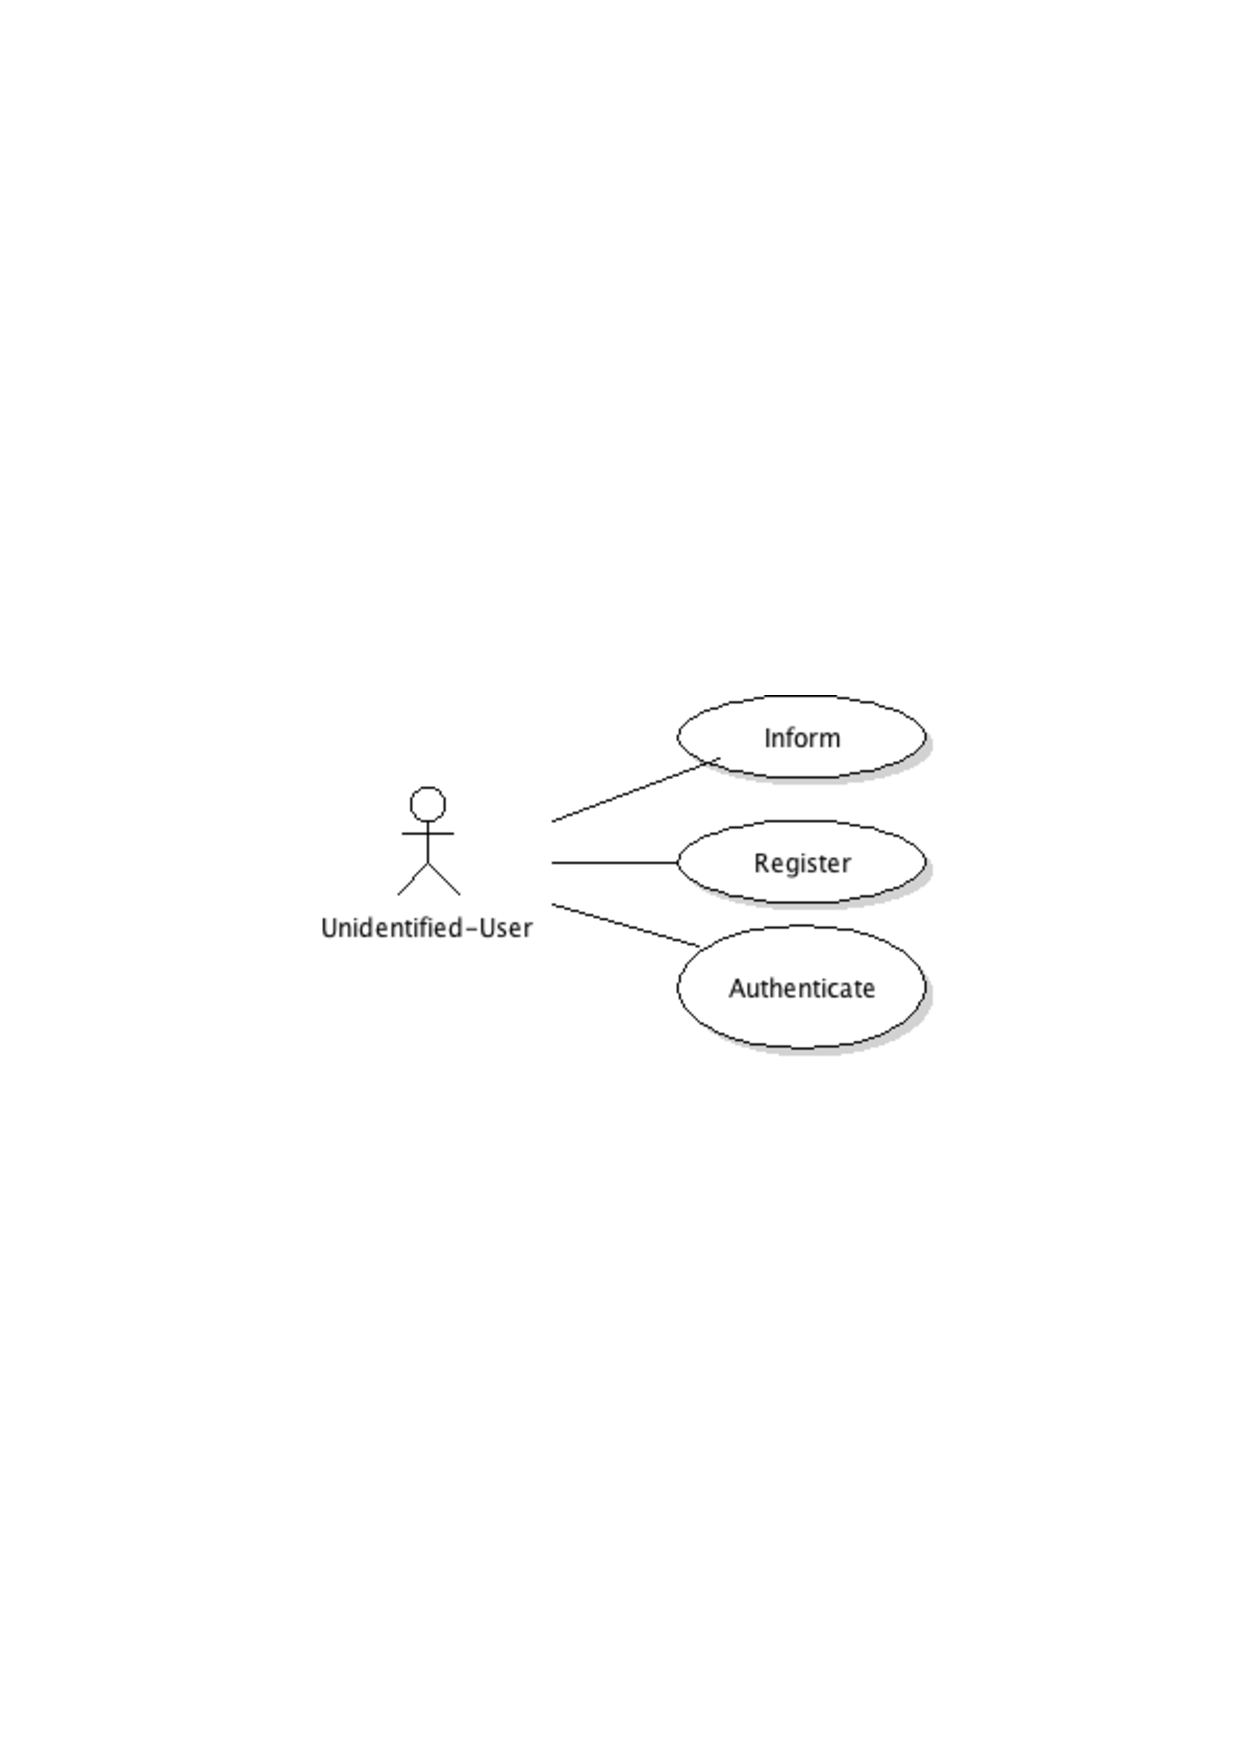
\includegraphics[width=\textwidth,  trim=2cm 12cm 2cm 11cm]{UML_figure/UC/uni_user/UC_UniUser_General.pdf}
				\caption{Unidentified user Use Case : Overview}
			\end{center}
		\end{figure}
	\subsection{Inform}An unidentified user will inform himself about the platform.
	\subsection{Register}An unidentified user who wants to access to the different features of the platform will have to register first.
	\subsection{Authenticate}An unidentified user authenticates to have access to the features if he has already passed the register step.
%end free user section
\newpage
%begin student section
\section{Student}
	\subsection{Overview}
		\begin{figure}[ht]
			\begin{center}
				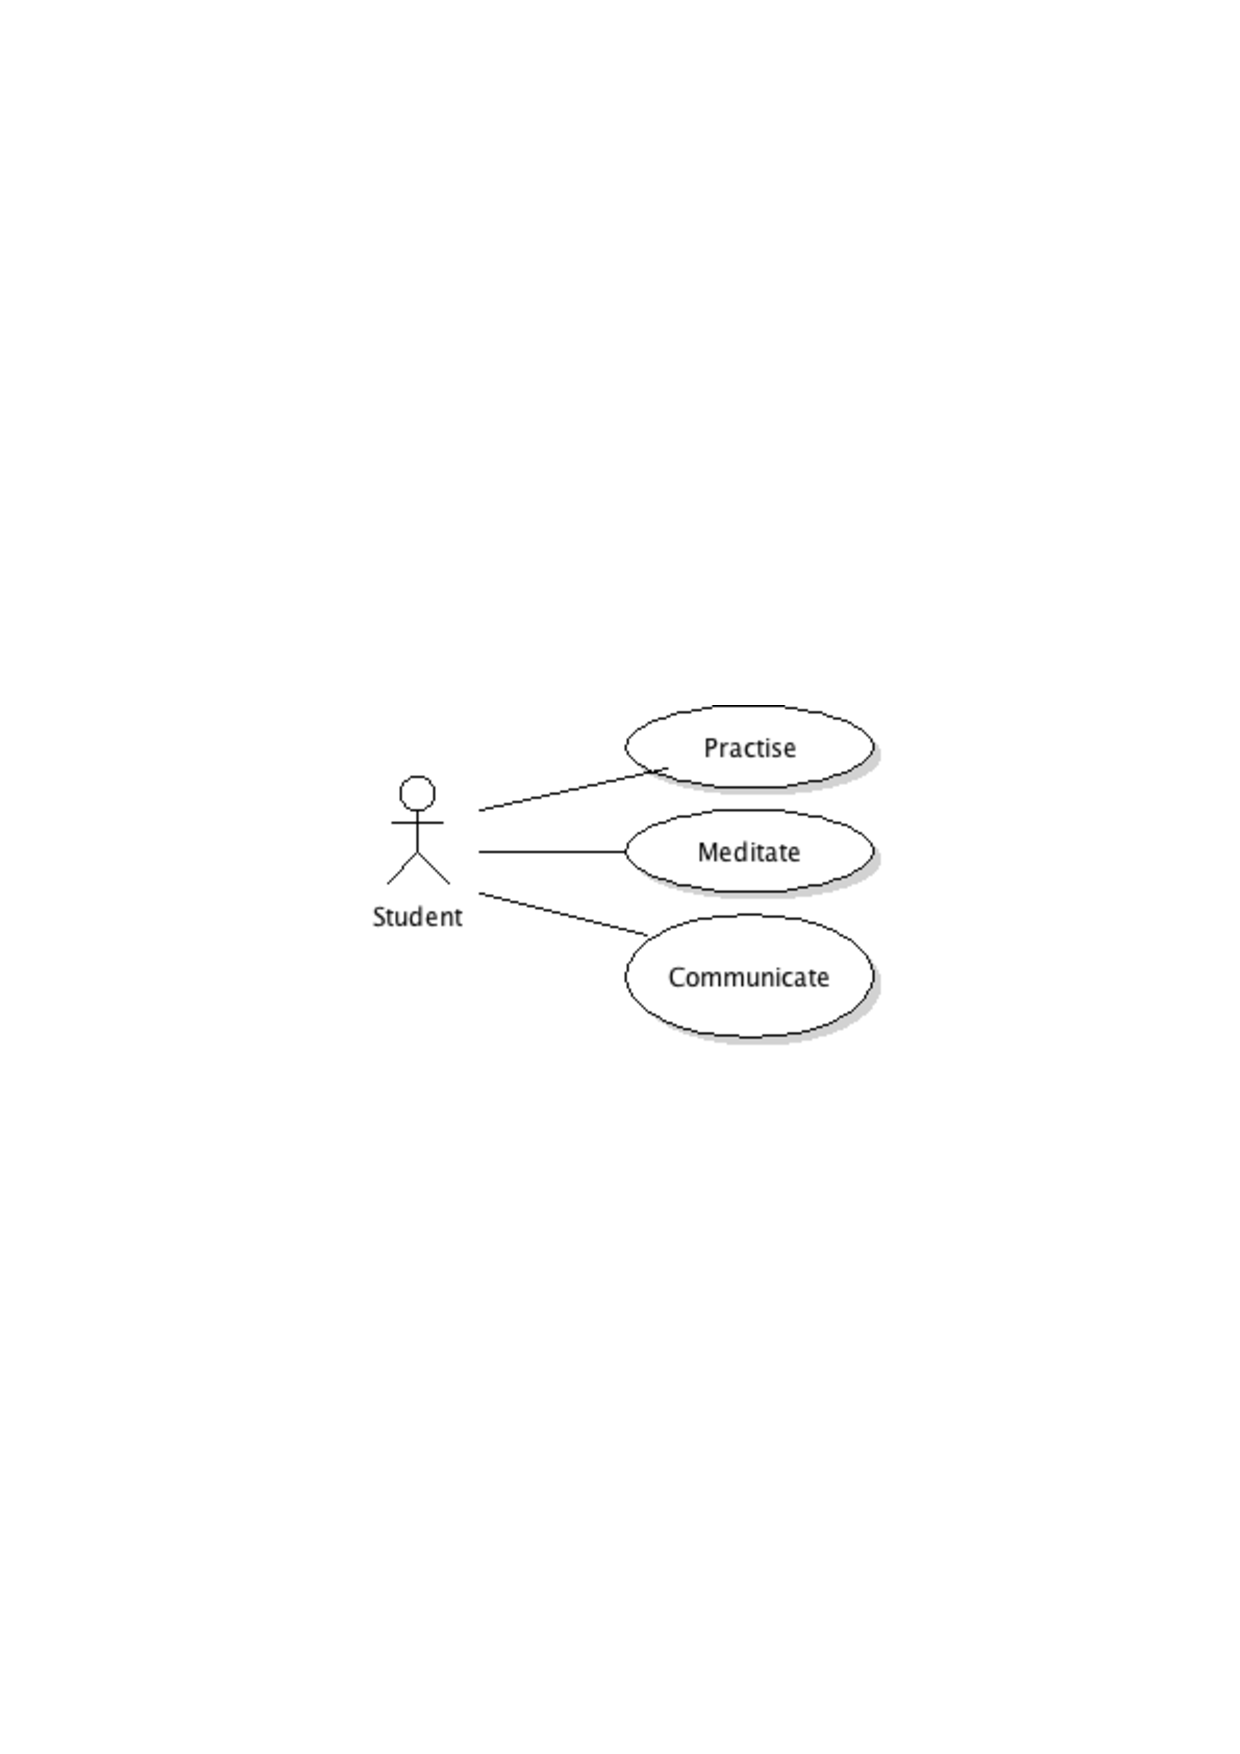
\includegraphics[width=\textwidth,  trim=2cm 12cm 2cm 11cm]{UML_figure/UC/student/UC_Student_General.pdf}
				\caption{Student Use Case : Overview}
			\end{center}
		\end{figure}
	\subsection{Practise}
		\begin{figure}[ht]
			\begin{center}
				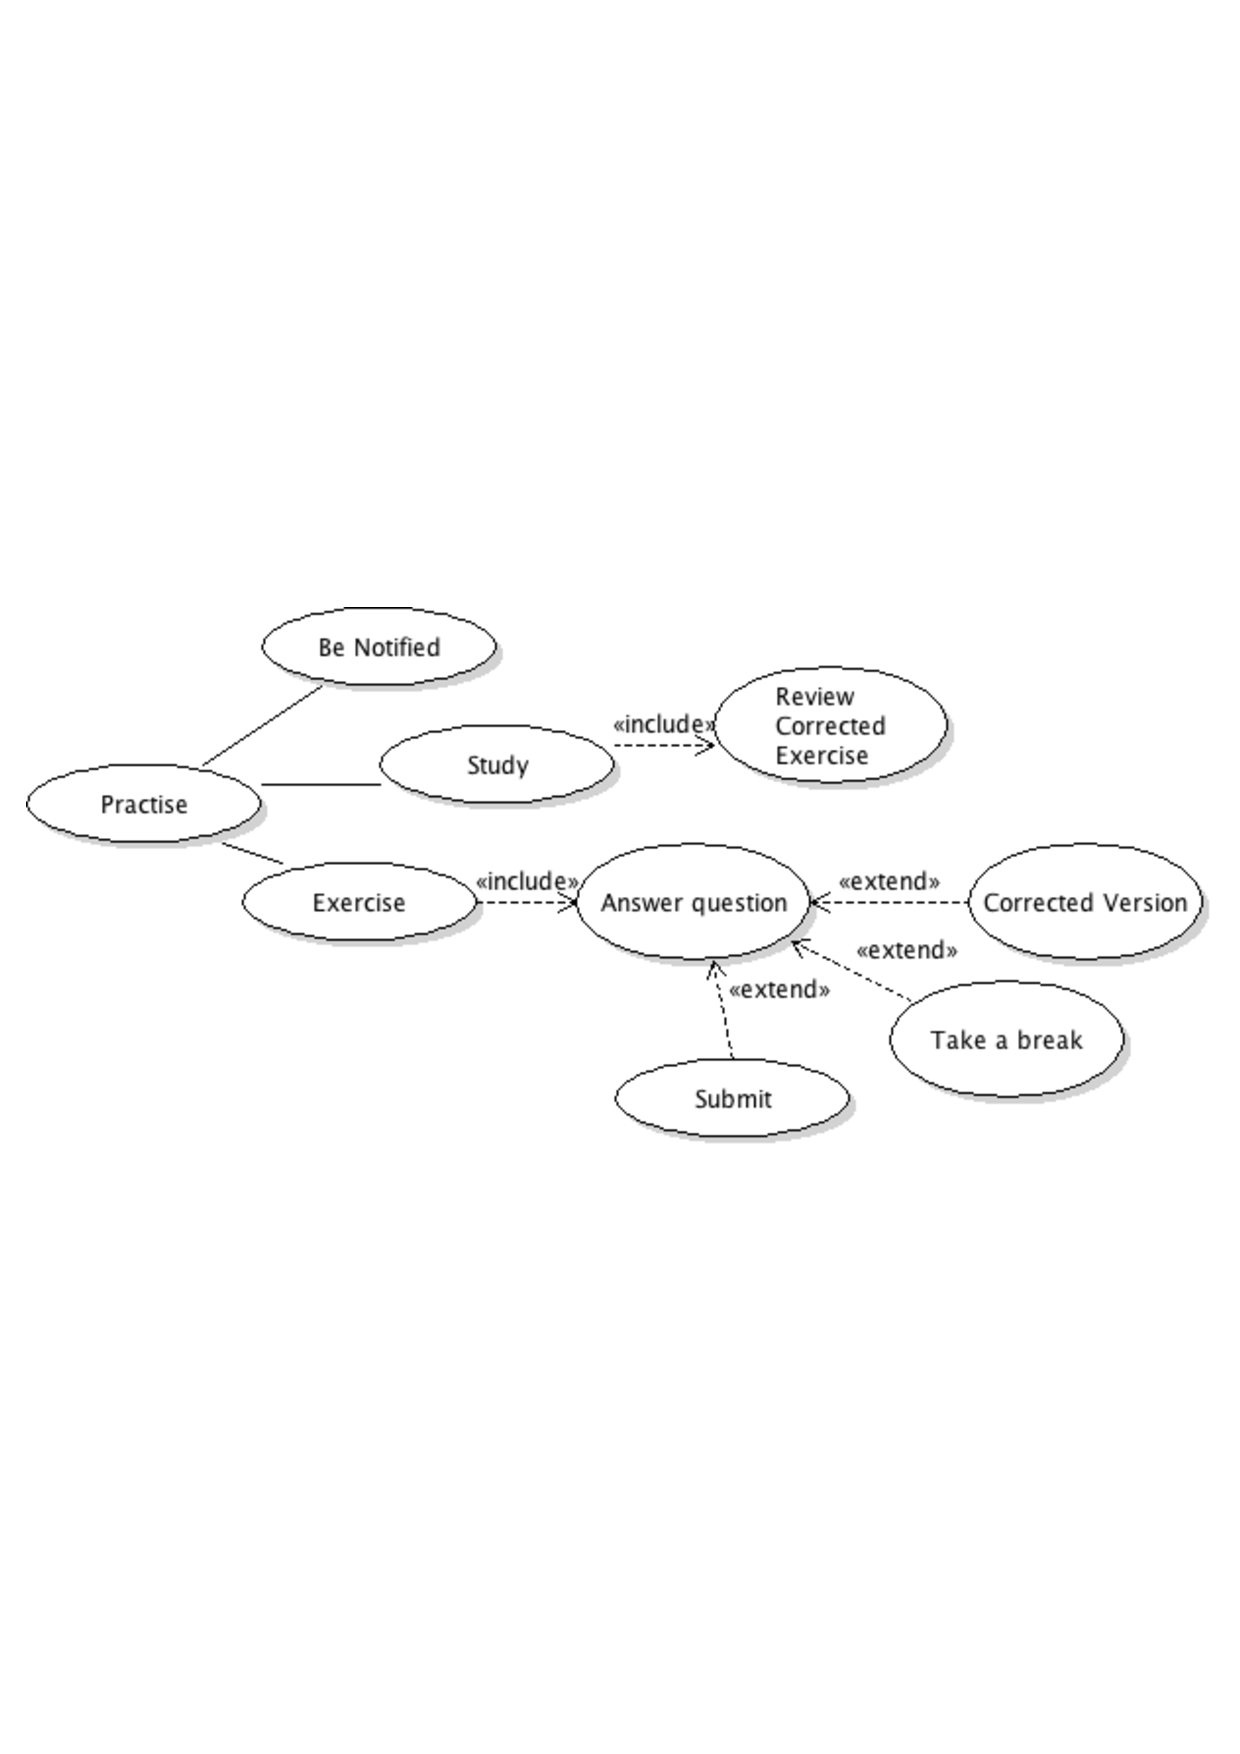
\includegraphics[width=\textwidth,  trim=2cm 10cm 2cm 10cm]{UML_figure/UC/student/UC_Student_Practise.pdf}
				\caption{Student Use Case : Practise}
			\end{center}
		\end{figure}
		\subsubsection{Be notified}
			The student will be notified for new events.
		\subsubsection{Study}
			The student can study by reviewing corrected exercises.
		\subsubsection{Exercise}
			The student can exercise himself by doing exercises written by the teacher.
		\subsubsection{Answer Question}
			The student will answer a set of different type of question.
		\subsubsection{Corrected Version}
			The student will have optionally access to the corrected version.
		\subsubsection{Take a break}
			The student can take a break and resume the exercise later.
		\subsubsection{Submit}
			The student can submit his answer form and be graded by the platform.		
	\subsection{Meditate}
		\begin{figure}[ht]
			\begin{center}
				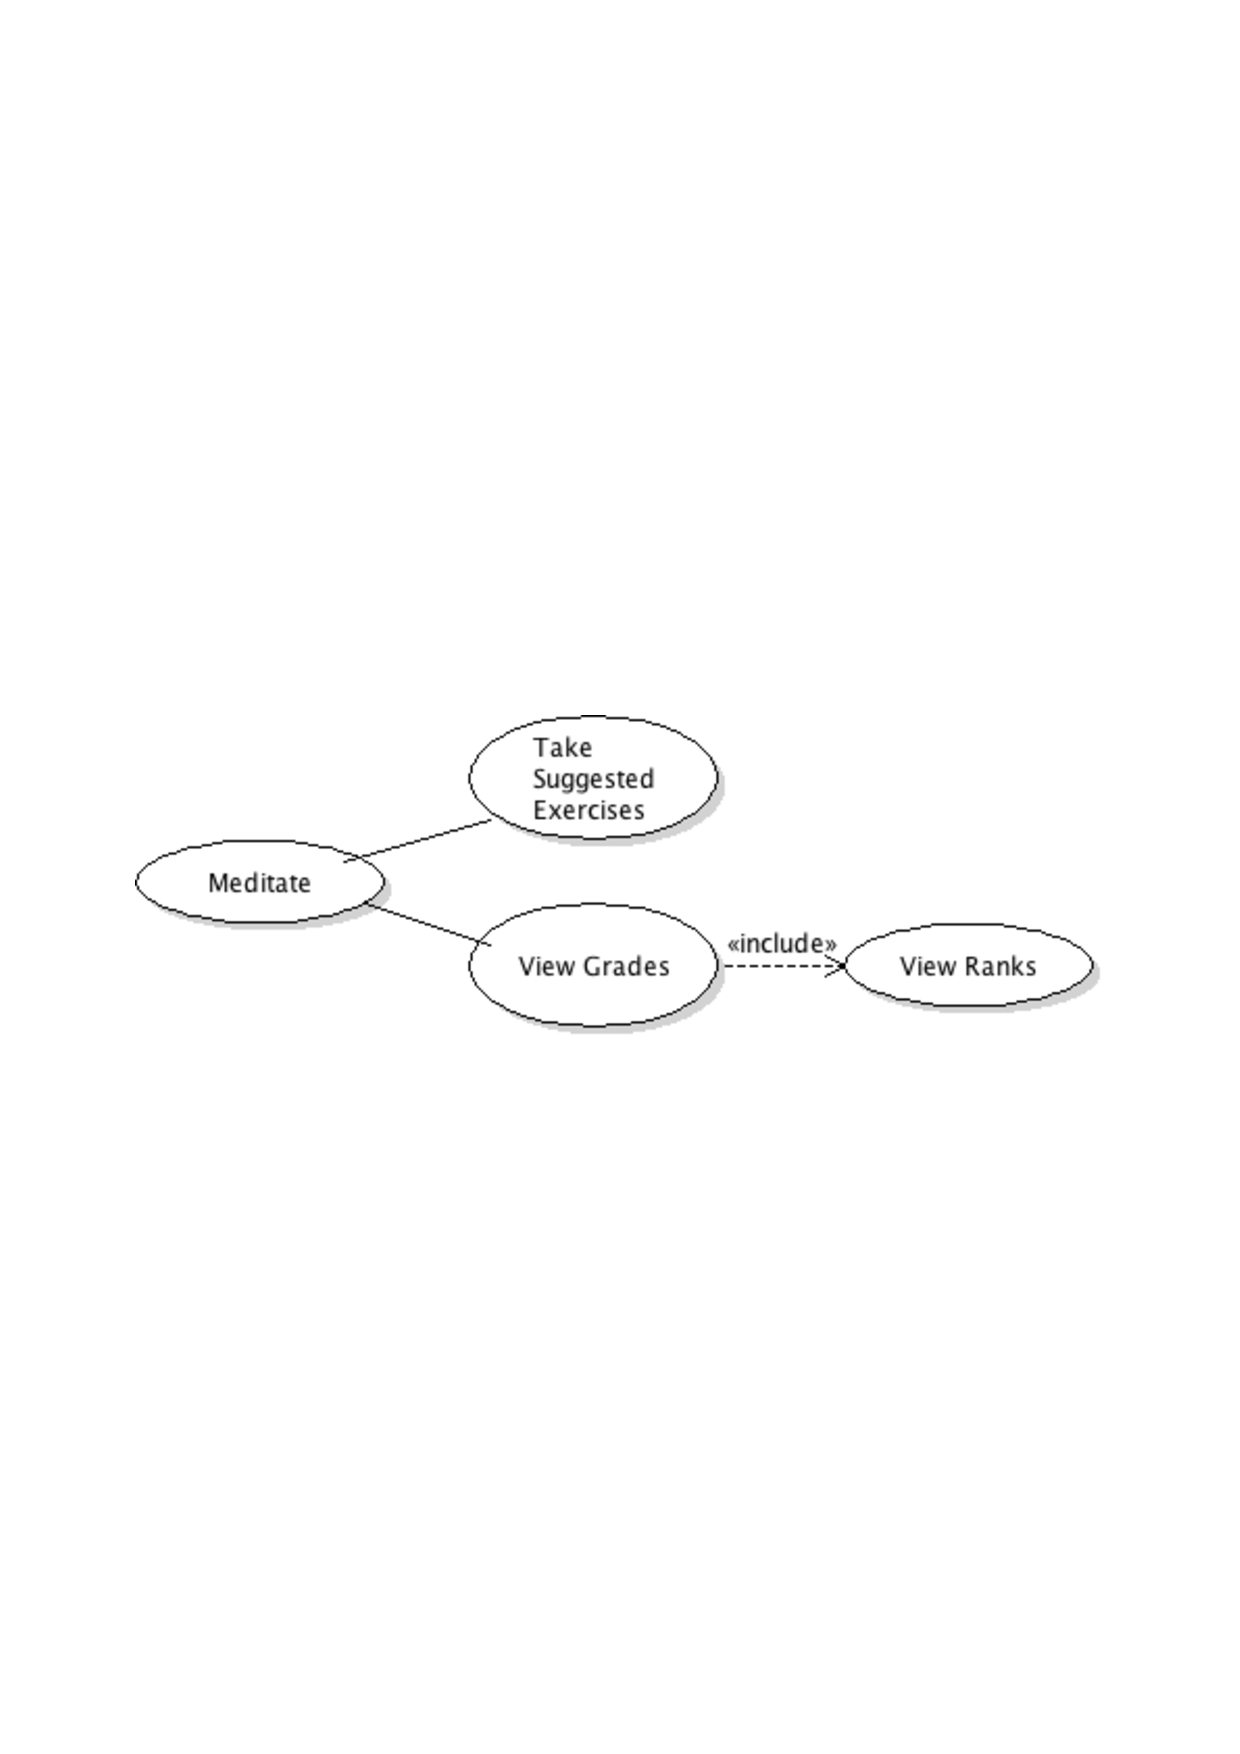
\includegraphics[width=\textwidth,  trim=2cm 12cm 2cm 12cm]{UML_figure/UC/student/UC_Student_Meditate.pdf}
				\caption{Student Use Case : Meditate}
			\end{center}
		\end{figure}
		\subsubsection{Take suggested exercises}
			The student can access and take a set of exercises according to their grade.
		\subsubsection{View Grades}
			The student can see their grade for each exercises.
		\subsubsection{View Ranks}
			The student can compare himself with other student.
%end student section
\newpage
%begin teacher section
\section{Teacher}
	\subsection{Overview}
		\begin{figure}[ht]
			\begin{center}
				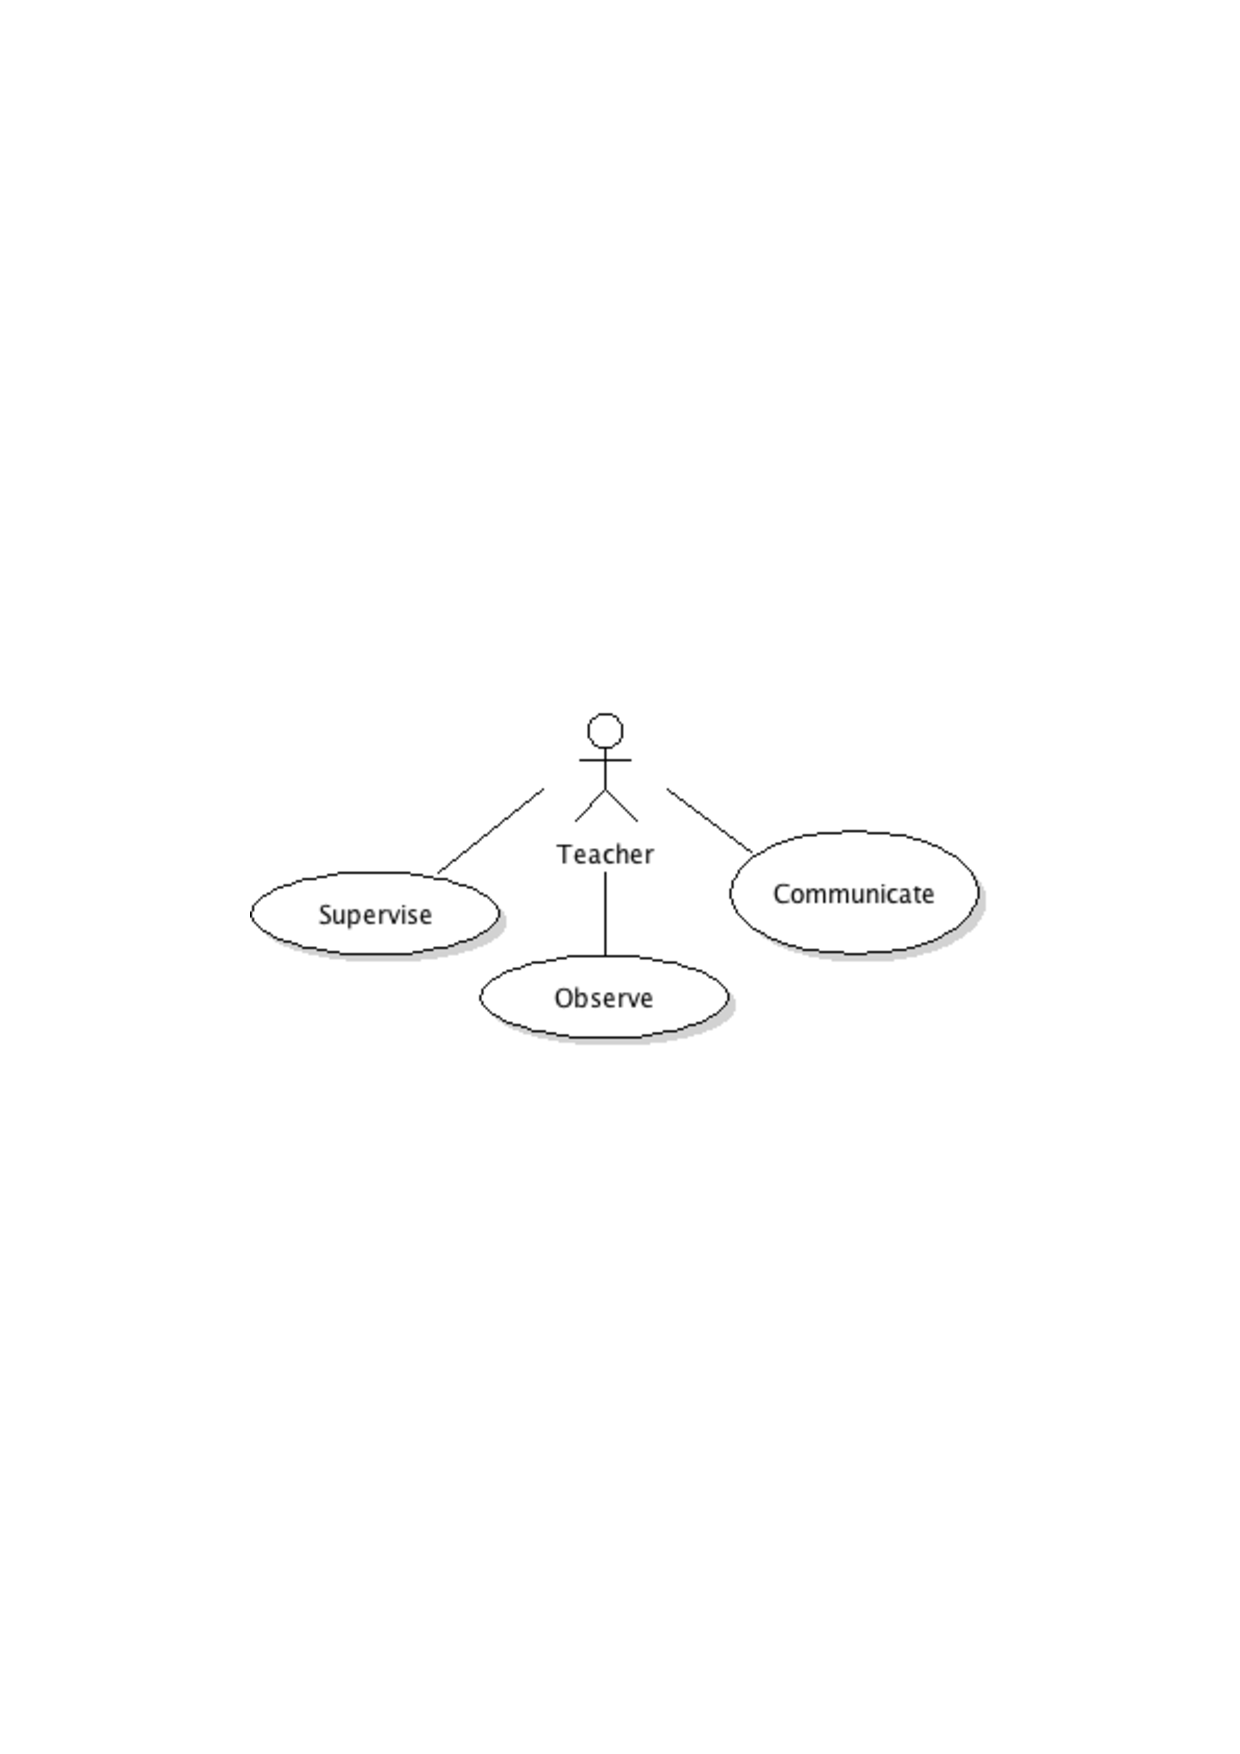
\includegraphics[width=\textwidth,  trim=2cm 11cm 2cm 12cm]{UML_figure/UC/teacher/UC_Teacher_General.pdf}
				\caption{Teacher Use Case : Overview}
			\end{center}
		\end{figure}
	\subsection{Supervise}
		\begin{figure}[ht]
			\begin{center}
				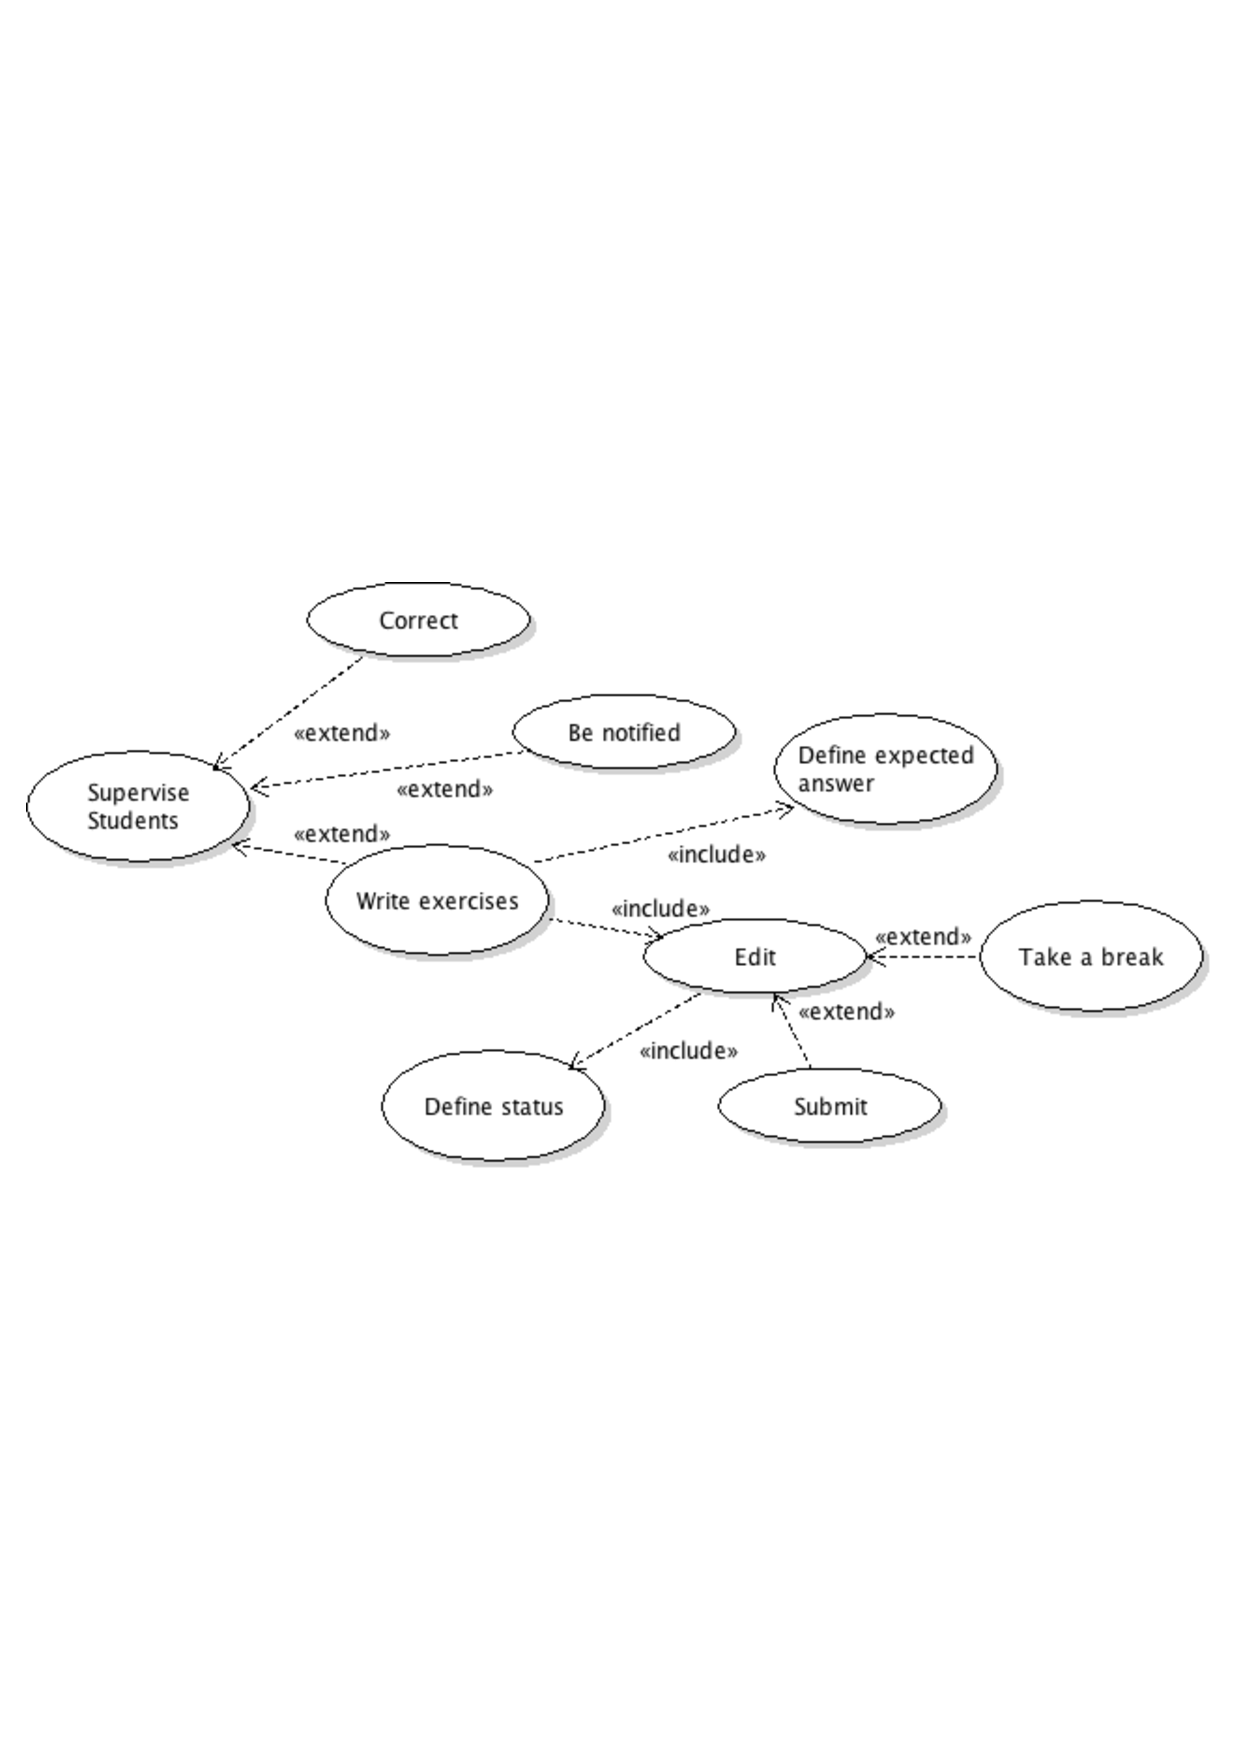
\includegraphics[width=\textwidth,  trim=2cm 10cm 2cm 10cm]{UML_figure/UC/teacher/UC_Teacher_Supervise.pdf}
				\caption{Teacher Use Case : Supervise}
			\end{center}
		\end{figure}
		\subsubsection{Correct}
			The teacher has to correct questions on which he has not define an answer.
		\subsubsection{Be Notified}
			The teacher will be notified by events.
			For instance the teacher will be notified when one of his exercises is online.
		\subsubsection{Write exercises}
			The teacher supervises his students by writing exercises.
		\subsubsection{Define expected answer}
			When the teacher writes exercises, he can optionally define an expected answer.
		\subsubsection{Edit}
			The teacher can edit an exercise written by him at anytime.
		\subsubsection{Define Status}
			The teacher can define status for his exercise such as date, deadline, priority.\\
			Release condition can also be defined. For instance, every student who have failed to complete the exercise 1.4 will be notified some other exercises. 
		\subsubsection{Take a break}
			The teacher can take a break about writing his exercise, to resume it later.
		\subsubsection{Submit}
			The teacher submit his exercise which can be viewed by student according to the exercise status defined by the teacher.
		
	\newpage
	\subsection{Observe}
		\begin{figure}[ht]
			\begin{center}
				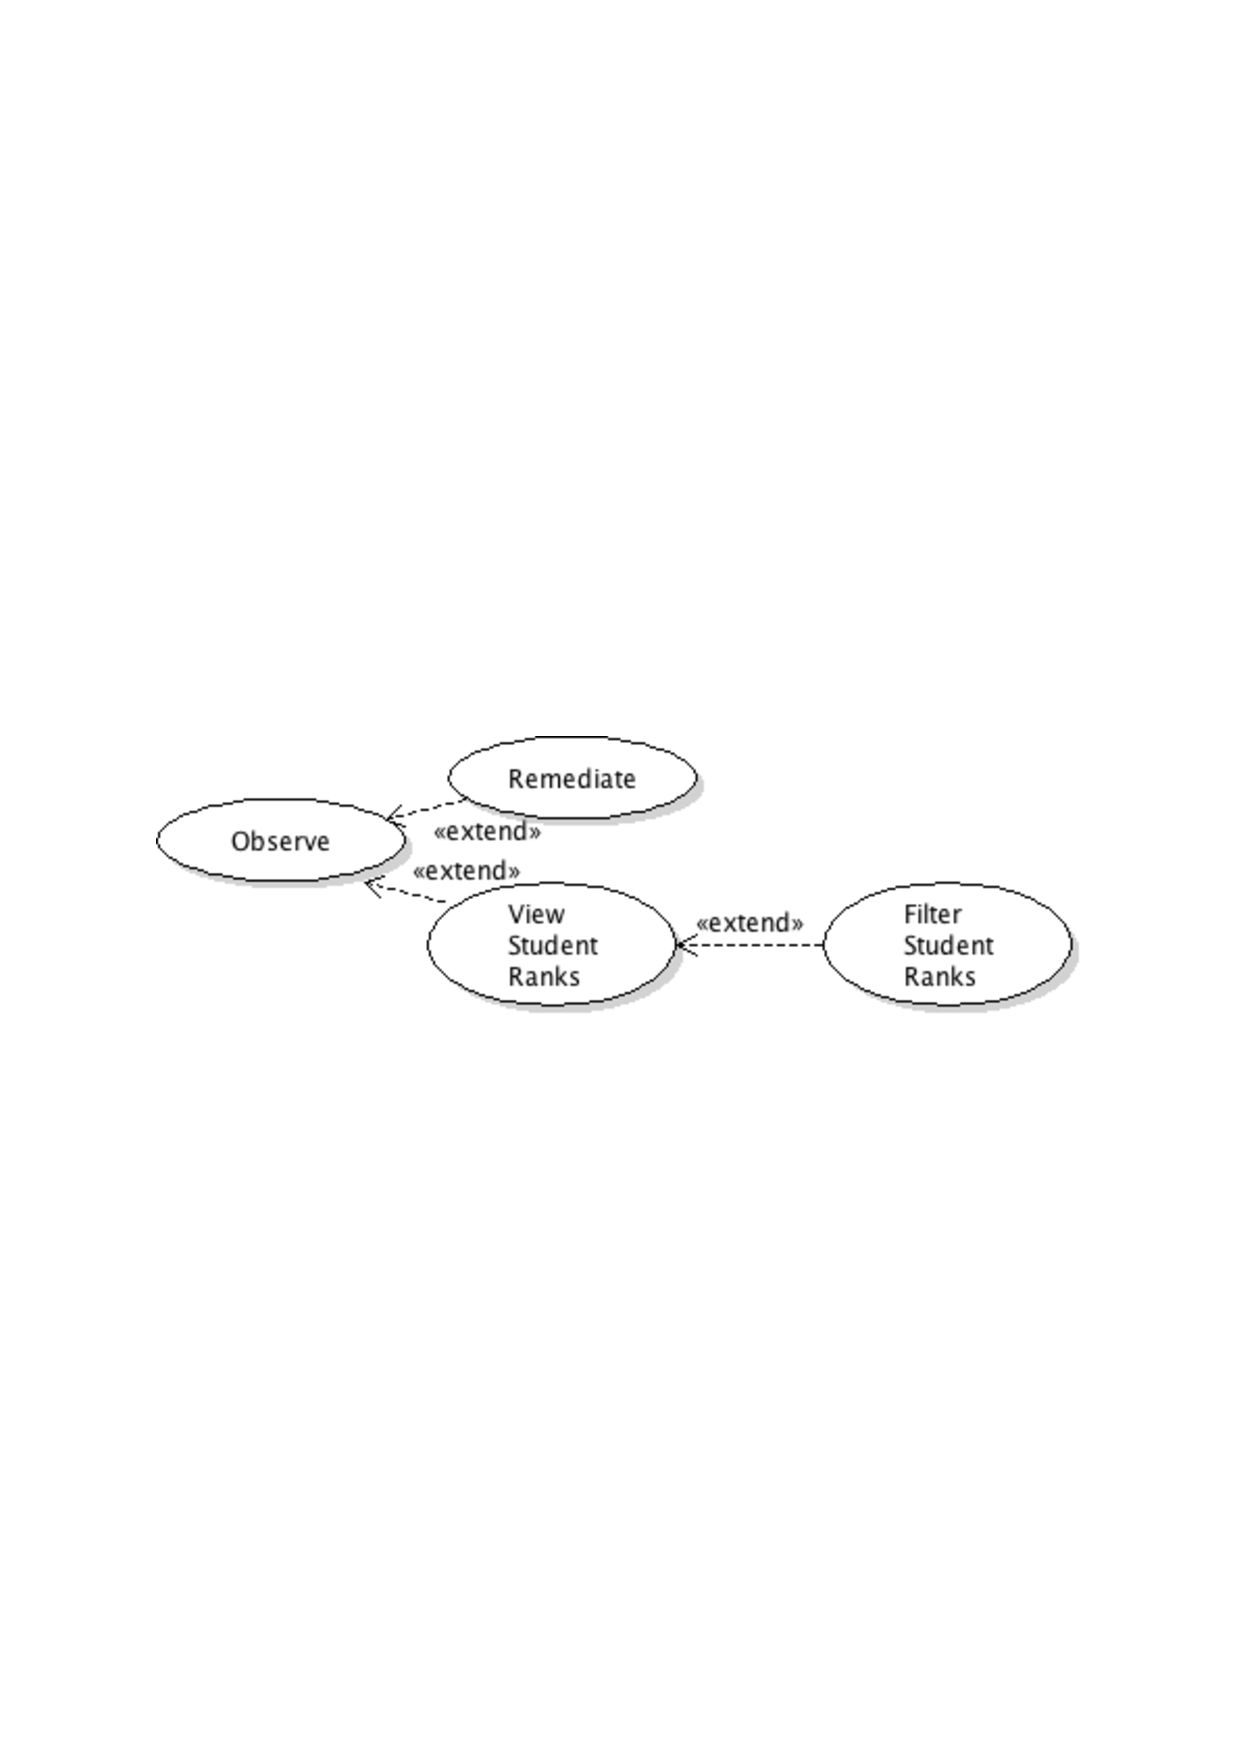
\includegraphics[width=\textwidth,  trim=2cm 12cm 2cm 12cm]{UML_figure/UC/teacher/UC_Teacher_Observe.pdf}
				\caption{Teacher Use Case : Observe}
			\end{center}
		\end{figure}
		\subsubsection{Rank}
			The teacher can see all the grades of students who took his exercises.
		\subsubsection{Filter}
			The teacher can filter the grades according to some parameters.
			The parameters can be the number of a group, the year.
		\subsubsection{Remediate}
			Then the teacher can provide exercises for a group of students in difficulties according to their grade.
%end teacher section
\newpage
%begin administrator section
\section{Administrator}
	\subsection{Overview}
		\begin{figure}[ht]
			\begin{center}
				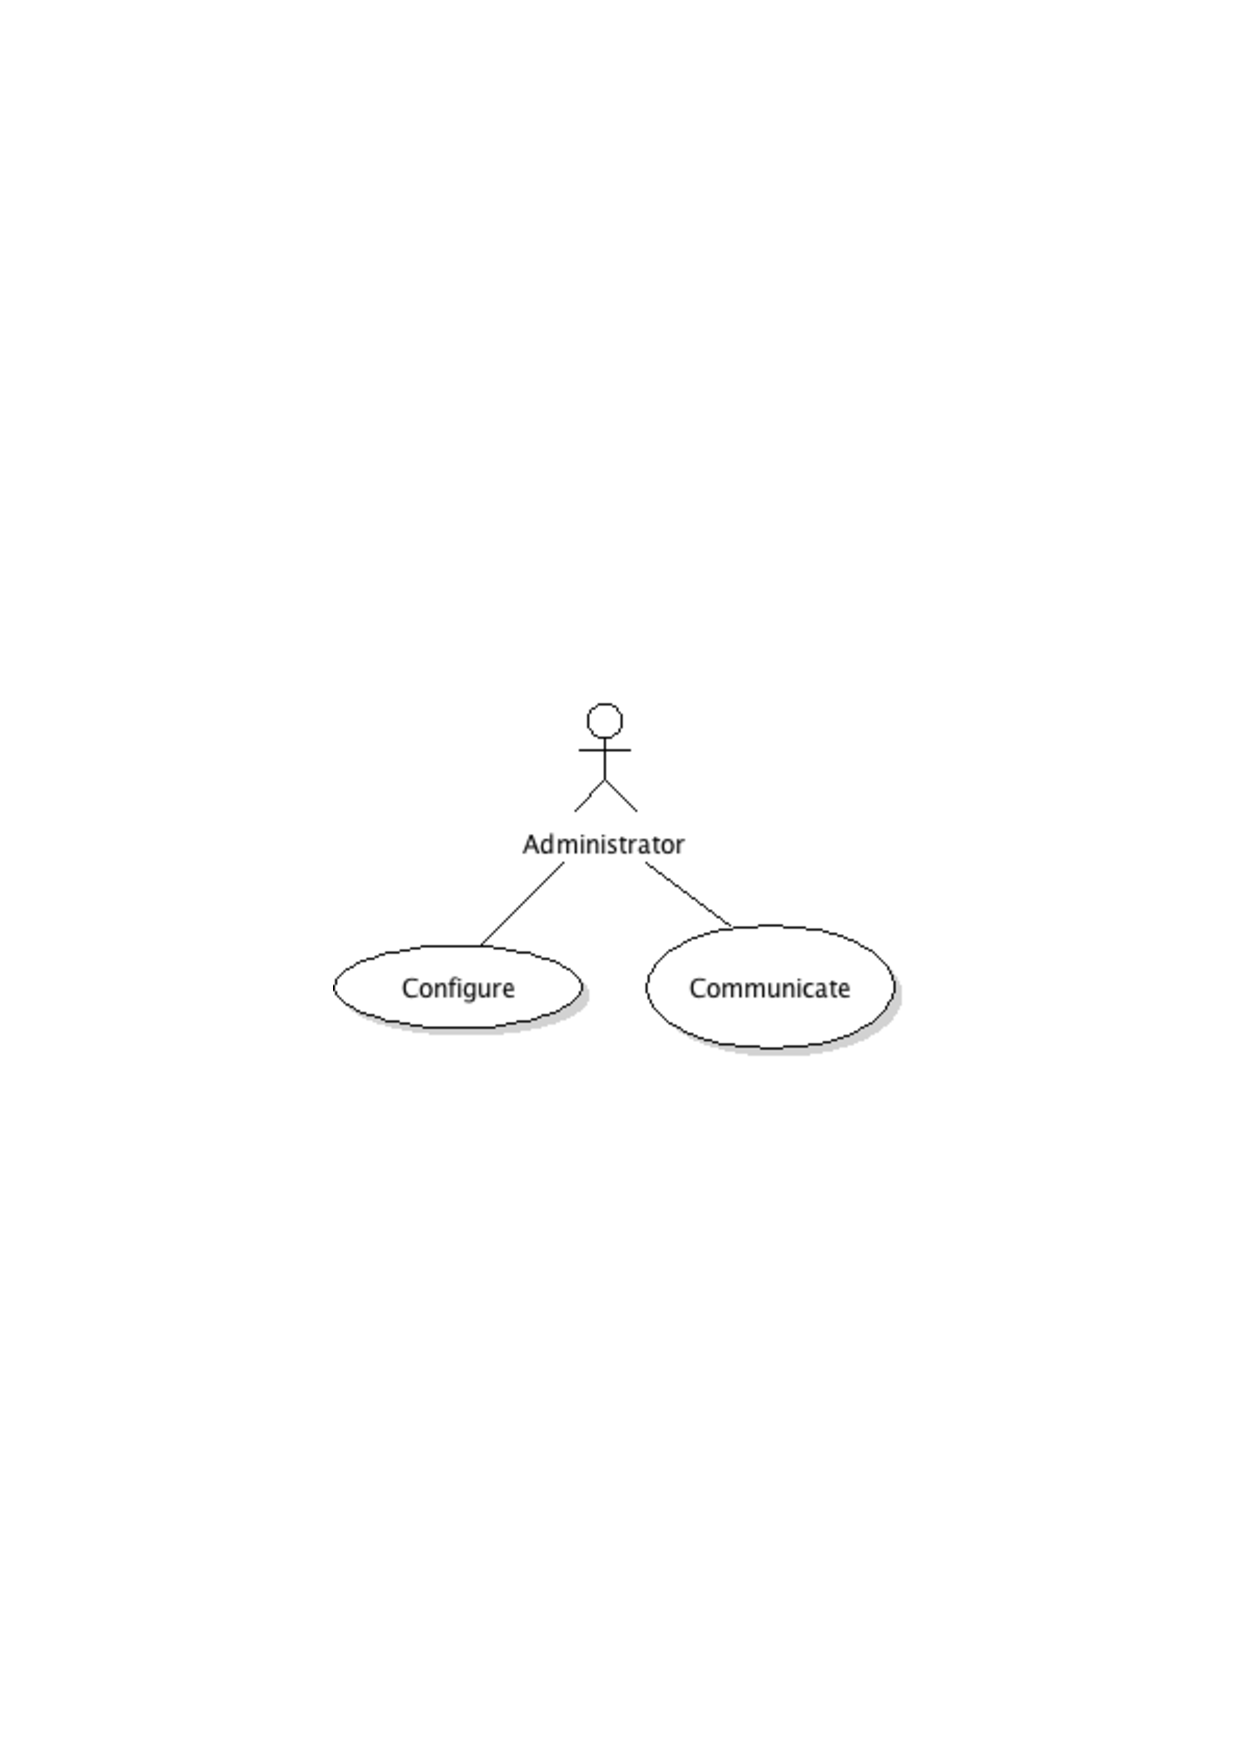
\includegraphics[width=\textwidth, trim=2cm 12cm 2cm 12cm]{UML_figure/UC/administrator/UC_Administrator_General.pdf}
				\caption{Administrator Use Case : Overview}
			\end{center}
		\end{figure}
	\subsection{Supervise the platform}
		\begin{figure}[ht]
			\begin{center}
				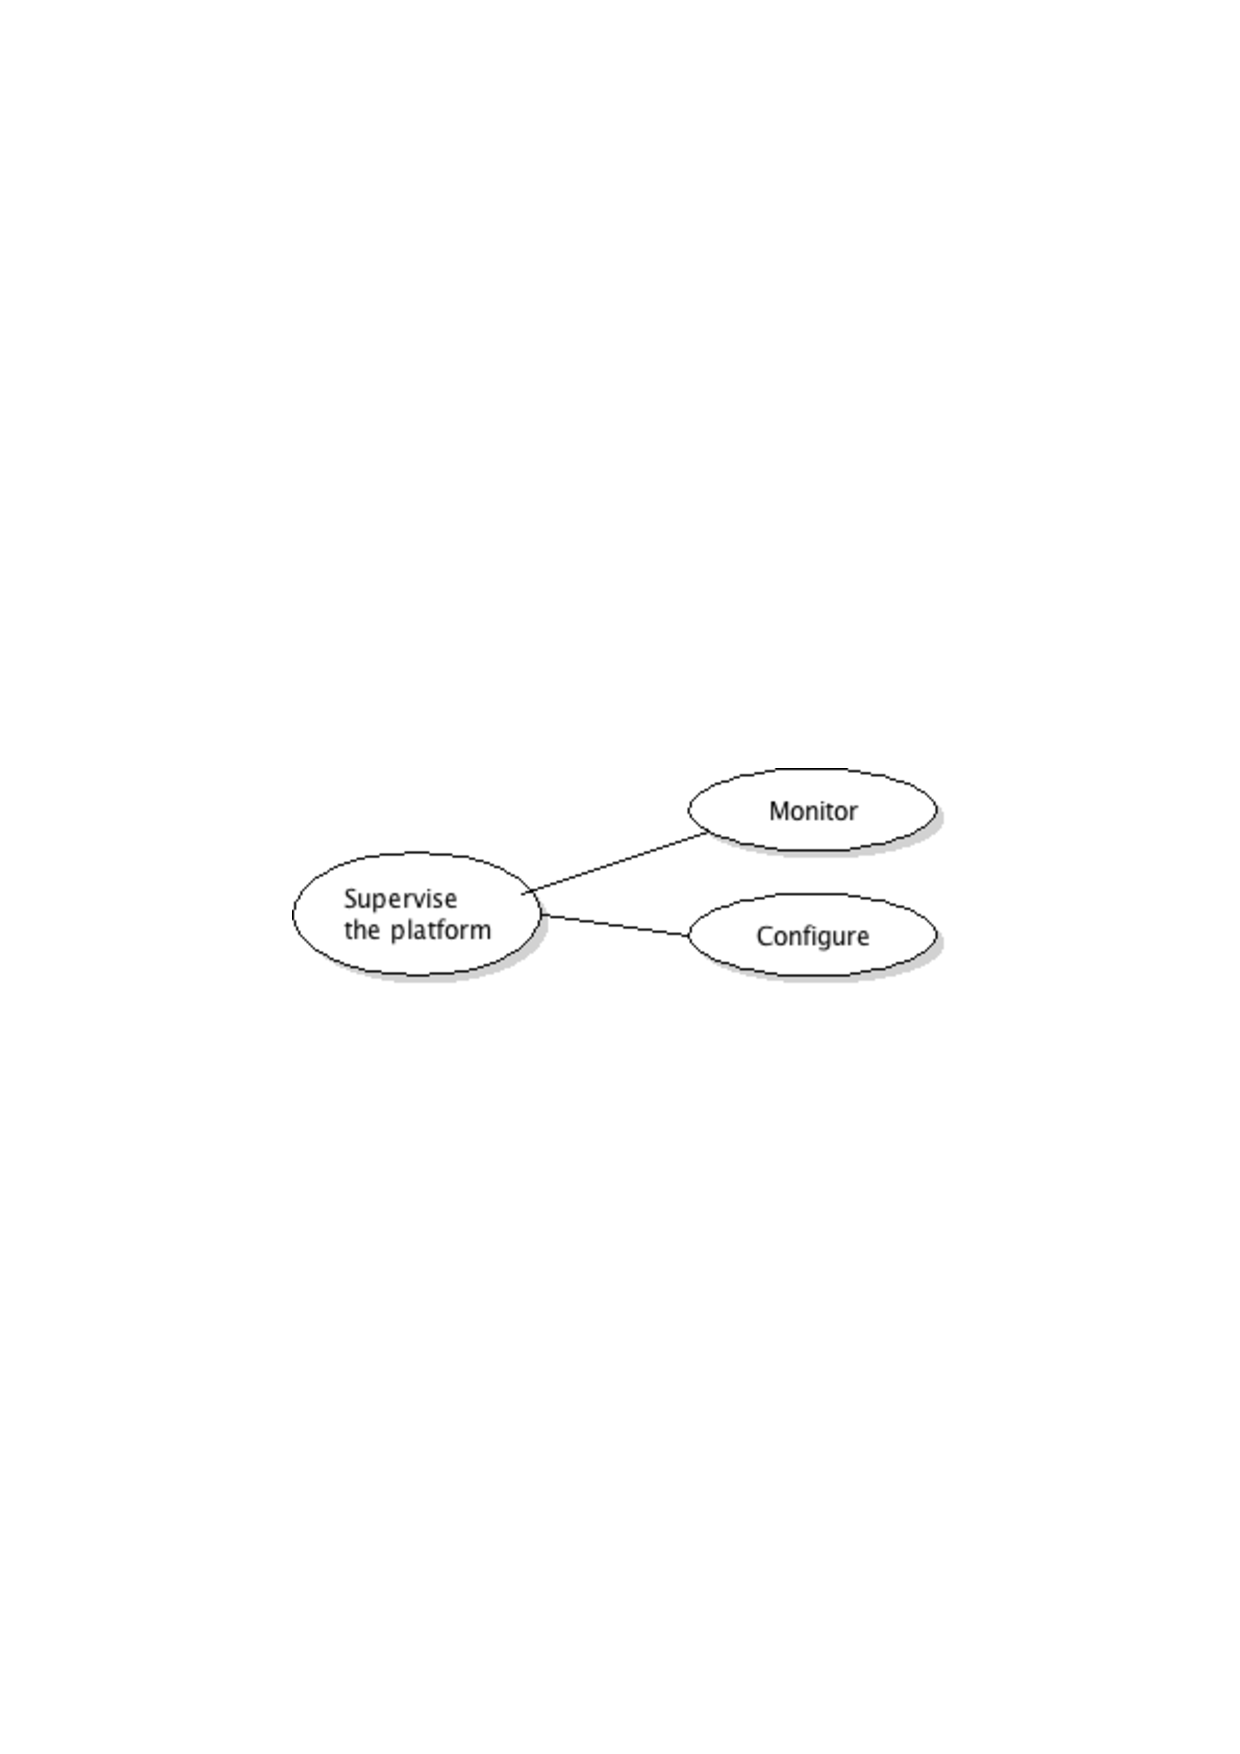
\includegraphics[width=\textwidth, trim=2cm 12cm 2cm 12cm]{UML_figure/UC/administrator/UC_Administrator_Supervise.pdf}
				\caption{Administrator Use Case : Overview}
			\end{center}
		\end{figure}
		\subsubsection{Monitor}
			The administrator can monitor the log.
		\subsubsection{Configure}
			The administrator can configure the platform.
%end administrator section
\newpage
%begin common user section
\section{Common registered user}
	\begin{figure}[ht]
		\begin{center}
			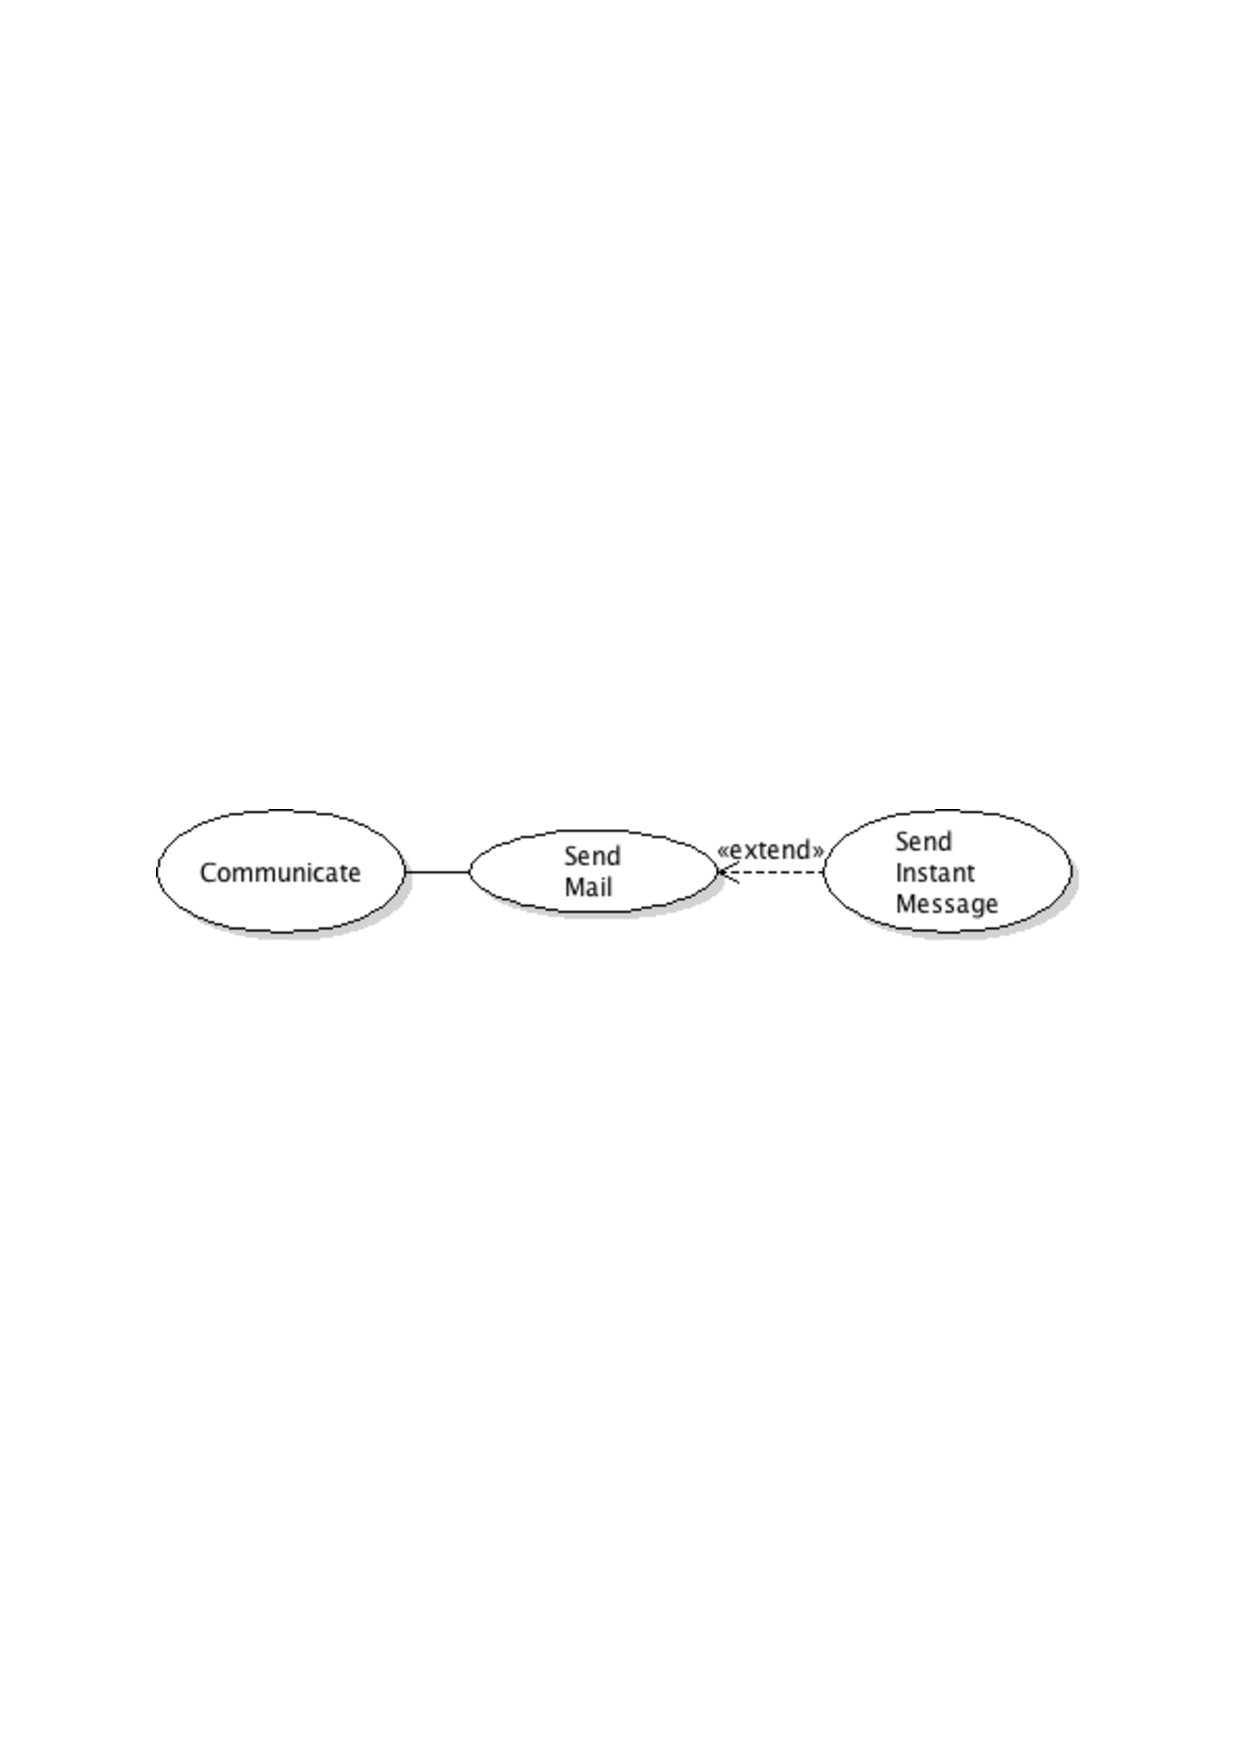
\includegraphics[width=\textwidth,  trim=2cm 12cm 2cm 12cm]{UML_figure/UC/common/UC_Common_Communicate.pdf}
			\caption{Registered user Use Case : Communicate}
		\end{center}
	\end{figure}
	\subsection{Communicate}
		\subsubsection{Send Mail}
			Identifed user communicate by mail exchange.
		\subsubsection{Send Instant Message}
			Identifed user communicate by instant message exchange.
%end common user section













